\documentclass[10pt,a4paper,twocolumn]{article}
\usepackage[T1]{fontenc}
\usepackage[utf8]{inputenc}
\usepackage[brazil]{babel}
\usepackage{mathptmx}
\usepackage[margin=1.5cm]{geometry}
\usepackage{graphicx}
\usepackage{booktabs}
\usepackage[font=small,labelfont=bf,skip=3pt]{caption}
\usepackage{enumitem}
\usepackage[small,compact]{titlesec}
\titlespacing*{\section}{0pt}{6pt}{3pt}
\usepackage[hidelinks]{hyperref}
\graphicspath{{../resultados/}}
\setlength{\columnsep}{0.6cm}
\setlist{nosep,leftmargin=*}
\renewcommand{\arraystretch}{0.95}
\newcommand{\cod}[1]{\texttt{\small #1}}
\pagestyle{empty}

\begin{document}
\twocolumn[{%
\begin{center}
{\large\bfseries T2 --- Mestre/escravo com MPI: busca de hiperparâmetros de uma MLP}\\[2pt]
Marina Bon e Heloysa Pelizon \quad|\quad
Repositório: \url{https://github.com/heloysapelizon/MLP-comp-par-t2}
\end{center}
\vspace{2pt}}]

\section{Modelagem}
O problema é uma busca de hiperparâmetros de uma rede MLP no MNIST, sobre o código C++/Eigen
do MLP-From-Scratch~[1]. A tarefa $i$ treina uma rede 784-$h$-$h$-10 por 2 épocas (lote 8),
com $h\in\{16,32\}$, taxa $\eta\in\{0{,}05;\,0{,}1;\,0{,}2\}$, semente $i$ e uma de 50 fatias
de 100 imagens de treino, tudo derivado de $i$ (\cod{tarefa.cpp:37}), e devolve os acertos em
200 imagens de teste (\cod{tarefa.cpp:48}). As tarefas são independentes e têm dois custos
($h=16$ ou 32). O saco são os índices $0..N-1$; cada escravo lê o MNIST antes da região medida,
então uma mensagem de tarefa leva só \{início, qtd\}: 8 bytes.

Há quatro tags (\cod{mestre\_escravo.cpp:18--23}): \cod{TAG\_PEDIDO} (escravo$\to$mestre,
vazia), \cod{TAG\_TAREFA} (\{início, qtd\}), \cod{TAG\_RESULTADO} (\{início, qtd, acertos\ldots\})
e \cod{TAG\_FIM} (vazia). O escravo começa pedindo (l.~75), e cada resultado (l.~90) vale como
novo pedido. O mestre recebe com \cod{MPI\_ANY\_SOURCE} e \cod{MPI\_ANY\_TAG} (l.~45) e responde
a \cod{status.MPI\_SOURCE}. A ordem do saco é mantida porque o resultado traz o índice inicial e
é copiado para \cod{acertos[início..]} (l.~50). O último bloco leva \cod{min(g, restantes)}
(l.~61), o que vale para qualquer $P\ge2$ e qualquer $N$. Com o saco vazio, o mestre responde
\cod{TAG\_FIM} (l.~65) e só sai depois de encerrar todos os escravos (l.~41 e 66). A granularidade
$g$ (tarefas por mensagem) vem da linha de comando (l.~103). Toda execução imprime a soma dos
acertos e a \emph{ordem} $=\sum(i+1)\,\mathrm{acertos}[i]$ (\cod{tarefa.cpp:70}), que só coincide
se cada resultado voltou à sua posição. Os dois valores coincidiram com os da sequencial nas
230~execuções paralelas, inclusive em todos os tamanhos da fraca.

\section{Ambiente e metodologia}
Usamos os nós \cod{atlantica03} e \cod{atlantica04} (partição \cod{LAD\_geral}), sempre com
\cod{sbatch} e \cod{-{}-exclusive}. O \cod{lscpu} mostra um Xeon E5520 de 2,27~GHz com 2~soquetes
$\times$ 4~núcleos $\times$ 2~threads, ou seja, \textbf{8 núcleos físicos e 16 threads por nó},
e não os 2$\times$8 do enunciado. Por isso, há um processo por núcleo físico só até $P=16$;
$P=32$ usa o HT e $P=64$ põe 2~processos em cada thread.
O \cod{srun -{}-distribution=block} coloca $P/2$ processos em cada nó (ranks $0..P/2-1$ no
\cod{atlantica03}, com o mestre). Usamos \cod{-{}-hint=nomultithread} até 8 processos por nó,
\cod{multithread} com 16 e \cod{-{}-overcommit} com 32 (\cod{scripts/comum.sh:67}); o
\cod{-{}-cpu-bind=verbose} confirmou uma CPU diferente para cada rank.
As duas versões são compiladas pelo \cod{mpicxx} (g++~9.4.0) com \cod{-std=c++17 -O3 -DNDEBUG},
sem \cod{-march=native} e sem OpenMP (Eigen com uma thread); a sequencial não chama MPI.
Na versão MPI, todos os processos leem o MNIST, passam por um \cod{MPI\_Barrier}, e o mestre
mede com \cod{MPI\_Wtime} da barreira até a chegada do último resultado (l.~124, 125 e 54).
Na sequencial, mede-se só o laço das tarefas. A entrada de referência tem 4000~tarefas:
$T_1=42{,}07$~s (mín.~41,91; máx.~42,25), ou 10,5~ms por tarefa. Na fraca, $N=4000\,P$, com o
mesmo custo por tarefa; as amostras treinadas, impressas em cada execução, vão de 1,6~M ($P=2$)
a 51,2~M ($P=64$), exatamente $P\times0{,}8$~M. Fizemos 10~repetições por configuração, com a
ordem das configurações alternada a cada repetição (\cod{comum.sh:40}).

\begin{table}[t]
\centering\footnotesize\setlength{\tabcolsep}{3.5pt}
\caption{Escalabilidade forte ($N=4000$, $g=1$): mediana [mín.--máx.] de 10 execuções.
$t_{\mathrm{tar}}$ é o tempo de cálculo por tarefa nos escravos; ocup.\ é a fração do tempo
em que os escravos calcularam.}
\label{tab:forte}
\begin{tabular}{@{}rcccrc@{}}
\toprule
$P$ & $T_P$ (s) & $S$ & $E$ & $t_{\mathrm{tar}}$ (ms) & ocup. \\
\midrule
1 (seq.) & 42,07 [41,91--42,25] & -- & -- & 10,5 & -- \\
2 & 42,87 [42,61--43,05] & 0,98 & 0,49 & 10,5 & 0,98 \\
4 & 14,22 [14,17--14,25] & 2,96 & 0,74 & 10,5 & 0,99 \\
8 & 6,44 [6,41--6,46] & 6,53 & 0,82 & 11,1 & 0,99 \\
16 & 3,63 [3,61--3,64] & 11,59 & 0,72 & 13,4 & 0,99 \\
32 (HT) & 4,04 [4,01--4,09] & 10,42 & 0,33 & 30,9 & 0,99 \\
64 (2/thread) & 4,36 [4,34--4,41] & 9,64 & 0,15 & 58,9 & 0,85 \\
\midrule
8 em 1 nó & 7,50 [7,48--7,55] & 5,61 & 0,70 & 13,1 & 1,00 \\
\bottomrule
\end{tabular}
\end{table}

\begin{table}[t]
\centering\footnotesize\setlength{\tabcolsep}{3.5pt}
\caption{Escalabilidade fraca ($N=4000\,P$, $g=1$): mediana [mín.--máx.] de 10 execuções,
$E_{\mathrm{fraca}}=T_1/T_P$.}
\label{tab:fraca}
\begin{tabular}{@{}rrcccc@{}}
\toprule
$P$ & $N$ & $T_P$ (s) & $E_{\mathrm{fraca}}$ & $t_{\mathrm{tar}}$ (ms) & ocup. \\
\midrule
2 & 8000 & 85,60 [84,91--86,32] & 0,49 & 10,5 & 0,98 \\
4 & 16000 & 56,71 [56,45--56,88] & 0,74 & 10,5 & 0,99 \\
8 & 32000 & 51,22 [50,99--51,31] & 0,82 & 11,1 & 0,99 \\
16 & 64000 & 57,64 [57,48--57,70] & 0,73 & 13,4 & 0,99 \\
32 & 128000 & 129,72 [129,08--130,32] & 0,32 & 31,2 & 0,99 \\
64 & 256000 & 278,53 [277,13--279,26] & 0,15 & 59,6 & 0,87 \\
\bottomrule
\end{tabular}
\end{table}

\section{Granularidade e balanceamento}
A Tab.~\ref{tab:gran} resume a varredura com $P=32$. Uma tarefa custa 10,5~ms sozinha e 31~ms
com $P=32$. A ida e volta de uma mensagem do mesmo tamanho ($g=1$) leva 1,0~$\mu$s dentro do nó e
193~$\mu$s entre nós, o que dá uma razão computação/comunicação de 55 no pior caso (tarefa
sequencial, entre nós) e de 160 com $P=32$. Agrupar tarefas economizaria no máximo 193~$\mu$s a cada
31~ms (0,6\%). O $g=1$ teve a menor mediana (4,04~s) e é o escolhido (\cod{comum.sh:20}).
Como $g=1$ é a unidade indivisível, a comparação é com granularidades maiores: $g$ de 2 a 128
ficou de 6 a 11\% mais lento, e $g=256$ e 512, 2,4 e 4,9 vezes mais lentos. A perda grande vem
do fim do saco. A ociosidade média no fim passa de 17~ms com $g=1$ (meia tarefa) para 0,29~s
com $g=32$, e chega a 7 e 17~s com $g=256$ e 512, quando só há 16 e 8 blocos para 31 escravos.
A diferença entre $g=1$ e $g=2..128$ não vem das mensagens, que pesariam no máximo 0,6\%: o
próprio cálculo por tarefa sobe de 31,0 para 32,3--32,9~ms, e não identificamos a causa. Uma
primeira varredura, com as configurações sempre na mesma ordem, deu o mesmo resultado.

Com $g=1$ e $P=32$, todos os escravos ficaram ocupados cerca de 4,0~s, mas o número de tarefas
depende de onde cada um roda. No \cod{atlantica03}, os escravos do soquete~0 (o do mestre)
fizeram 138--140 tarefas; o rank~2, que divide o núcleo físico com o mestre (CPUs 0 e 8 no
\cod{lscpu -e}), fez 171; os do soquete~1 fizeram 121--125. No \cod{atlantica04}, onde não há
mestre, cada escravo fez de 124 a 128. O mestre passa quase todo o tempo esperando e deixa o
núcleo e o soquete mais livres, ou seja, \emph{o custo de uma tarefa depende de quantos
processos calculam no mesmo núcleo e soquete}. O saco sob demanda compensou essas diferenças:
no fim, a espera média foi de meia tarefa.

\begin{table*}[t]
\centering\footnotesize\setlength{\tabcolsep}{5pt}
\caption{Granularidade com $P=32$ e $N=4000$: tempo total, mensagens de resultado, ociosidade
média dos escravos no fim do saco e ida e volta (pingpong) de uma mensagem do mesmo tamanho.
Mediana [mín.--máx.] de 10 execuções.}
\label{tab:gran}
\begin{tabular}{@{}rcrccc@{}}
\toprule
$g$ & $T_{32}$ (s) & mensagens & ocioso no fim (s) & ida e volta no nó ($\mu$s) & ida e volta entre nós ($\mu$s) \\
\midrule
1 & 4,04 [3,99--4,07] & 4000 & 0,02 & 1,00 [0,97--1,04] & 193 [143--222] \\
2 & 4,26 [4,23--4,34] & 2000 & 0,02 & 1,00 [0,96--1,02] & 193 [139--222] \\
4 & 4,31 [4,23--4,37] & 1000 & 0,05 & 0,97 [0,96--1,02] & 192 [140--222] \\
8 & 4,28 [4,22--4,36] & 500 & 0,08 & 0,97 [0,95--1,02] & 193 [144--222] \\
16 & 4,40 [4,17--4,52] & 250 & 0,22 & 1,01 [1,00--1,06] & 194 [145--224] \\
32 & 4,45 [4,37--4,67] & 125 & 0,29 & 1,11 [1,09--1,14] & 196 [146--225] \\
64 & 4,47 [4,38--4,52] & 63 & 0,26 & 1,46 [1,42--1,52] & 200 [146--227] \\
128 & 4,48 [4,44--4,56] & 32 & 0,28 & 1,49 [1,46--1,53] & 205 [153--229] \\
256 & 9,87 [6,40--14,76] & 16 & 6,99 & 1,71 [1,68--1,73] & 213 [159--234] \\
512 & 19,93 [11,05--26,80] & 8 & 17,04 & 1,97 [1,84--1,98] & 228 [169--244] \\
\bottomrule
\end{tabular}
\end{table*}

\begin{figure*}[t]
\centering
\begin{minipage}[t]{0.485\textwidth}\centering
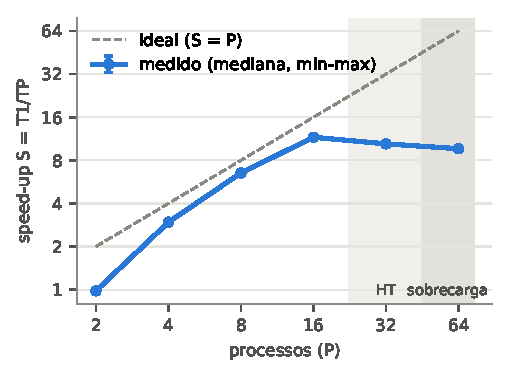
\includegraphics[width=\linewidth]{speedup.pdf}
\caption{Speed-up da forte (mediana, barras de mín.--máx.) e reta ideal. As faixas marcam o
HT ($P=32$) e 2 processos por thread ($P=64$).}
\label{fig:speedup}
\end{minipage}\hfill
\begin{minipage}[t]{0.485\textwidth}\centering
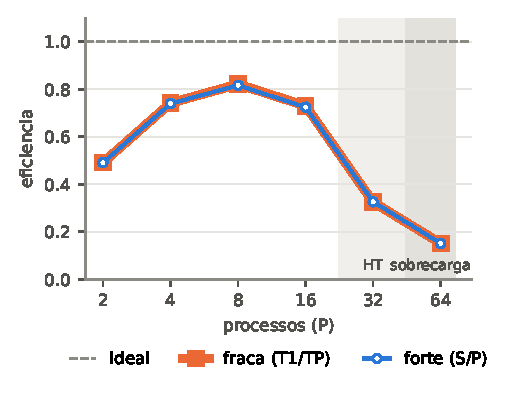
\includegraphics[width=\linewidth]{eficiencia.pdf}
\caption{Eficiência da forte ($S/P$) e da fraca ($T_1/T_P$). As duas curvas se sobrepõem.}
\label{fig:eficiencia}
\end{minipage}
\end{figure*}

\section{Análise dos resultados}
A eficiência se decompõe em três fatores medidos,
$E=\frac{P-1}{P}\cdot\frac{t_{\mathrm{seq}}}{t_{\mathrm{tar}}(P)}\cdot\mathrm{ocup.}$
(Tabs.~\ref{tab:forte} e~\ref{tab:fraca}); por exemplo, com $P=16$:
$0{,}94\times0{,}78\times0{,}99=0{,}72$. Cada fator corresponde a uma causa:
\begin{itemize}
\item \textbf{Núcleo do mestre.} Com $P=2$, $S=0{,}98$ e $E=0{,}49$: o único escravo calcula
  quase como a sequencial (eficiência por escravo de 0,98), mas metade dos núcleos é do mestre.
\item \textbf{Comunicação.} Com $P=2$, o escravo fica no outro nó, e a diferença
  $42{,}87-42{,}07=0{,}80$~s corresponde a $4000\times0{,}19$~ms $=0{,}77$~s de idas e voltas.
  Até $P=32$ a ocupação fica em 0,98 ou mais, ou seja, comunicação e fim do saco custam 2\% ou
  menos. \emph{Dentro do nó contra entre nós:} $P=8$ num nó só, onde a comunicação é 190 vezes
  mais barata, levou 7,50~s, contra 6,44~s em dois nós, porque com 8 processos no nó cada
  tarefa custa 13,1~ms, e com 4, 11,1~ms.
\item \textbf{Disputa dentro do nó} (onde o speed-up satura). O tempo de cálculo por tarefa
  sobe de 10,5 para 13,4~ms com 8 processos por nó ($P=16$); a eficiência cai para 0,72 e o
  speed-up chega ao máximo, 11,6, em $P=16$ (Fig.~\ref{fig:speedup}). Isso é compatível com
  a disputa pelo L3 (8~MB por soquete) e pela memória, mas não medimos contadores de hardware
  para separar as duas.
\item \textbf{HT} ($P=32$). Com 2 processos por núcleo, cada tarefa leva 30,9~ms, 2,3 vezes os
  13,4~ms de $P=16$: cada núcleo rende 0,87 do que rendia com um processo. O HT não ajuda neste
  código; o speed-up cai para 10,4.
\item \textbf{Mestre como gargalo} ($P=64$). O tempo por tarefa dobra
  ($58{,}9\approx2\times30{,}9$~ms), como esperado com 2 processos por thread, e a ocupação cai
  de 0,99 para 0,85. Atribuímos essa queda ao mestre: ele divide uma thread com um escravo, e
  enquanto o sistema operacional executa o escravo, os pedidos dos outros 62 esperam. A mesma
  queda aparece na fraca (0,87).
\end{itemize}
\textbf{Fraca contra forte.} As curvas coincidem (Fig.~\ref{fig:eficiencia}), com diferença
de no máximo 0,006: as perdas estão no núcleo do mestre e no custo de cada tarefa, que não
dependem de $N$, e a comunicação e o fim do saco já custavam cerca de 1\% na forte. Por isso a
fraca não se sustenta melhor. A melhor configuração é $P=16$, com um processo por núcleo físico.

\section{Uso de ferramentas de IA}
Usamos o Claude Code (Anthropic) para escrever, a partir de um plano do grupo, a unidade de
trabalho, as versões sequencial e MPI, o pingpong, os scripts \cod{sbatch} e o
\cod{analise.py}; para diagnosticar, durante os experimentos, a topologia dos nós e a escolha
de $g$; e para redigir um rascunho deste relatório. O grupo executou e conferiu todas as
medições na Atlântica, revisou o código e o texto e é capaz de explicá-los. Todos os números
vêm das saídas do Slurm guardadas em \cod{resultados/}.

\small
\noindent\textbf{Referências.} [1] muchlakshay, \emph{MLP-From-Scratch},
\url{https://github.com/muchlakshay/MLP-From-Scratch} (licença MIT).
[2] Y.~LeCun, C.~Cortes, C.~Burges, \emph{The MNIST database of handwritten digits}.
[3] Eigen~3.4, \url{https://eigen.tuxfamily.org}.

\end{document}
